\documentclass{article}
\usepackage{graphicx}
\usepackage{subfigure}
\usepackage{multirow}
\usepackage{wrapfig}
\usepackage{amssymb}
\usepackage{amsfonts, amsmath}
\usepackage{amsmath}
\usepackage{mathrsfs}
\usepackage{enumerate}
\usepackage[bookmarks=true]{hyperref}
% \usepackage[acronym]{glossaries}
%\usepackage{bookmark}
\usepackage{amssymb,amsmath,amsthm,amsfonts}
\usepackage{mathrsfs}
\usepackage{dsfont}
\usepackage{enumerate}

%\newtheorem{mdef}{Definition}
%\newtheorem{theorem}{Theorem}
\newcommand{\eqsplit}[2]{
  \begin{equation}\label{#2}
    \begin{split}
      #1
    \end{split}
  \end{equation}}
\newcommand{\eqnsplit}[1]{
  \begin{eqnarray*}
    #1
  \end{eqnarray*}}
\newcommand{\tran}[1]{
  \tilde{#1}
}
\newcommand{\td}[2]{
  \frac{d #1}{d #2}
}
\newcommand{\pd}[2]{
  \frac{\partial #1}{\partial #2}
}
\newcommand{\ppd}[2]{
  \frac{\partial^2 #1}{\partial #2^2}
}
\newcommand{\pdd}[3]{
  \frac{\partial^2 #1}{\partial #2 \partial #3}
}
\newcommand{\otd}[1]{
  \frac{d}{d #1}
}
\newcommand{\opd}[1]{
  \frac{\partial}{\partial #1}
}
\newcommand{\oppd}[1]{
  \frac{\partial^2}{\partial #1^2}
}
\newcommand{\opdd}[2]{
  \frac{\partial^2}{\partial #1 \partial #2}
}
\newcommand{\ket}[1]{
  |#1\rangle
}
\newcommand{\bra}[1]{
  \langle#1|
}
\newcommand{\inn}[1]{
  \langle#1\rangle
}
\newcommand{\mean}[1]{
  \langle#1\rangle
}
\newcommand{\tr}{
  \text{tr}\,
}
\newcommand{\re}{
  \text{Re}\,
}
\newcommand\im{
  \text{Im}\,
}
\newcommand{\var}{
  \text{var}
}
\newcommand{\arcsinh}{
  \sinh^{-1}
}
\newcommand{\arccosh}{
  \cosh^{-1}
}
\newcommand{\erfc}{
  \text{erfc}
}
\newcommand{\E}{
  \mathbb{E}
}
\renewcommand{\P}{
  \mathbb{P}
}
\newcommand{\I}[1]{
  \mathbf{1}_{\{#1\}}
}
\newcommand{\1}[1]{
  \mathds{1}_{\{#1\}}
}
\newcommand{\diag}{
  \text{diag\,}
}
\newcommand{\M}{
  {\text{max}}
}
\newcommand{\m}{
  {\text{min}}
}
\newcommand{\ph}{
  {\text{arg}\,}
}
\newcommand\erf{
  \text{erf}
}
\renewcommand\vec[1]{
  \mathbf{#1}
}
\newcommand\mtx[1]{
  \mathbf{#1}
}
\newcommand\ed{
  \,{\buildrel d \over =}\,
}




\DeclareGraphicsExtensions{.eps}
\title{Spectral properties of a Wishart-GARCH Matrix}
\author{Prof. Sven \AA berg\\
  Xie Xiaolei}
\begin{document}
\maketitle
\section{The Spectral Distribution}
\subsection{Dependence on auto-correlation}
Figure \ref{fig:spectral_dist} shows the spectral density of the
correlation matrix of N identically distributed GARCH(1,1)
processes. These processes have such parameters that 
the $\alpha_1 + \beta_1 \approx 1$ and hence the auto-correlation
function $\text{corr}(r^2_t, r^2_{t-k})$ decays with a similar slow
rate for all the processes but from different initial values. The
parameter settings also make these processes have very similar tail
behavior with a tail exponent $\alpha$ in the range $2.17 \pm 0.01$.

Figure \ref{fig:spectral_dist1} shows the central part of the spectral
distribution and figure \ref{fig:spectral_dist2} shows how the
Hellinger distance between the empirical spectral density and the
Marcenko Pastur law changes with the parameter $\alpha_1$.
It is seen that, when measured by the Hellinger metric, the empirical
spectral density is most similar to the Marcenko-Pastur law when
$\alpha_1 = 1/2$.
\begin{figure}[htb!]
  \centering
  \subfigure[Spectral density of the correlation matrix plotted on
  log-log scale. The mean is 1 for all the empirical distributions and
  also for the Marcenko-Pastur law.]{
    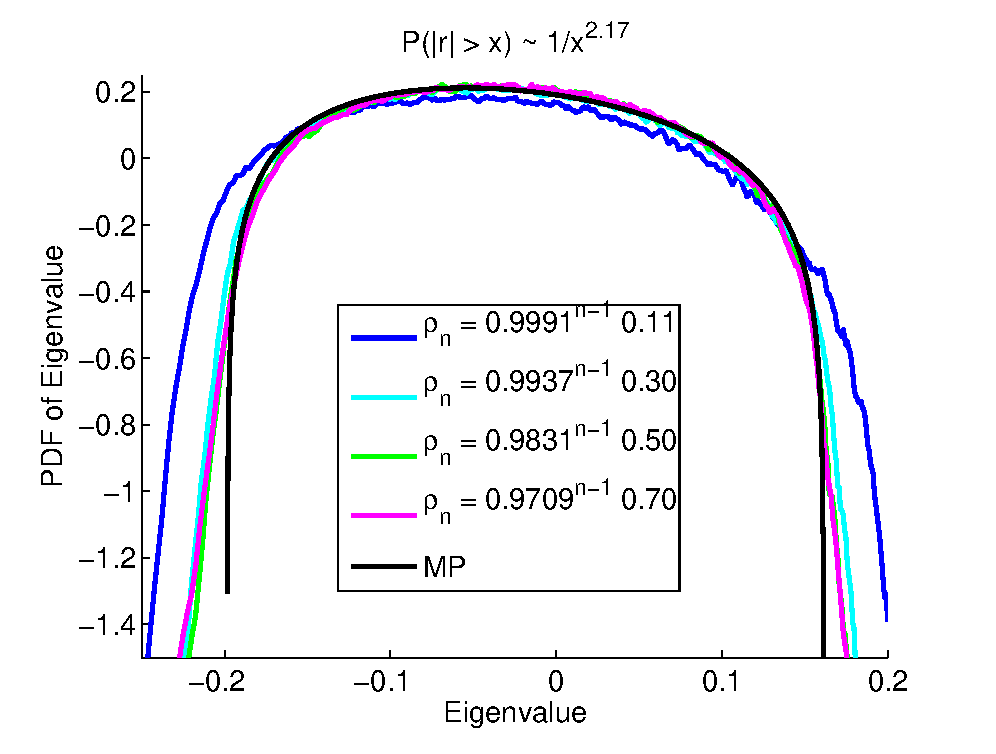
\includegraphics[scale=0.32]{../pics/spectral_dist2.eps}
    \label{fig:spectral_dist2}
  }
  \hspace{5mm}
  \subfigure[Hellinger distance between the empirical spectral density
  and the Marcenko-Pastur law.]{
    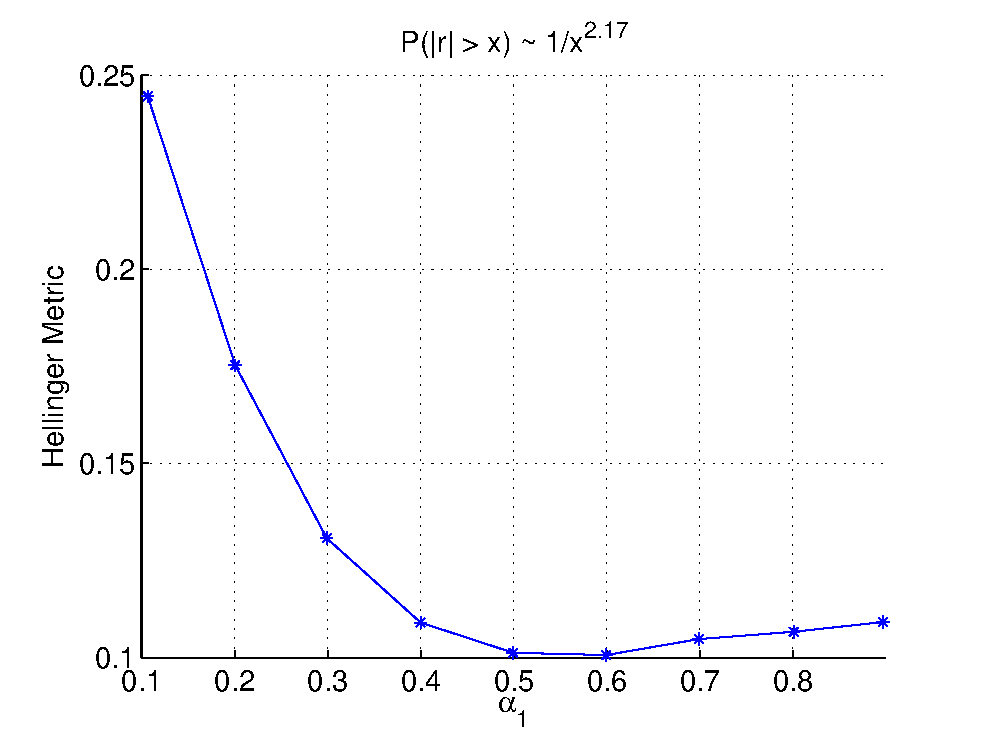
\includegraphics[scale=0.32]{../pics/spectral_dist1.eps}
    \label{fig:spectral_dist1}
  }
  \caption{\small \it Spectral density of the
    correlation matrix of N identically distributed GARCH(1,1)
    processes.}
  \label{fig:spectral_dist}
\end{figure}
On the other hand, it is also seen that the variance of the spectral
distributions decreases as auto-correlation becomes stronger. This is
further shown in figure \ref{fig:spectral_dist3}.
\begin{figure}[htb!]
  \centering
  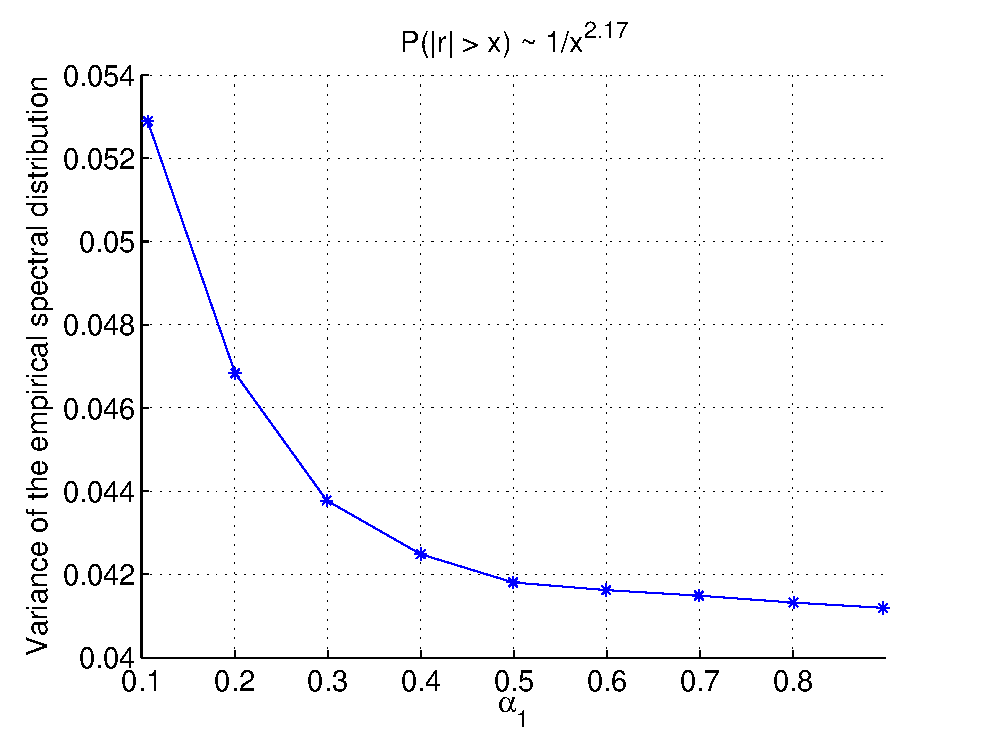
\includegraphics[scale=0.5]{../pics/spectral_dist3.eps}
  \caption{\small \it Variance of the spectral distributions.}
  \label{fig:spectral_dist3}
\end{figure}

\subsection{Dependence on the tail exponent}
Figure \ref{fig:spectral_density1} shows the dependence of the
spectral density of Wishart-GARCH matrices on the tail exponent
$\alpha$.
\begin{figure}[htb!]
  \centering
    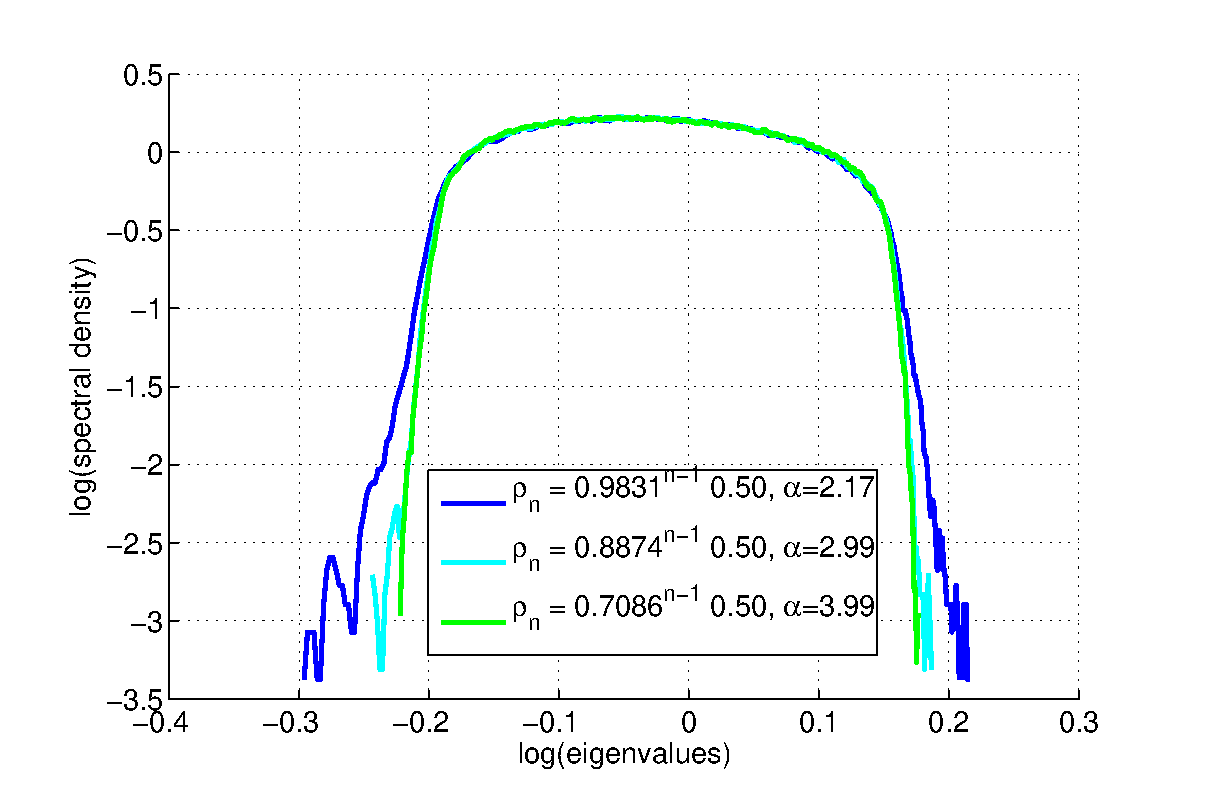
\includegraphics[scale=0.4]{../pics/spectral_density1.eps}
    \caption{\small \it Dependence of spectral density (plotted on
      log-log scale) on the tail exponent. The means of the 3
      distributions are all equal to 1 and the variances are all equal
      to 0.04}
    \label{fig:spectral_density1}
\end{figure}
The mean and variance of the three density functions as well as their
Hellinger distances to the Marcenko-Pastur law are as follows:
\begin{table}[htb!]
  \centering
  \begin{tabular}{|l|c|c|c|}
    \hline
    Tail Exponent & 2.17 & 2.99 & 3.99 \\
    \hline
    mean & 1.0000 & 1.0000 & 1.0000 \\
    \hline
    variance & 0.0418 & 0.0409 & 0.0408 \\
    \hline
    Hellinger distance & 0.1012 & 0.0639 & 0.0586 \\
    \hline
  \end{tabular}
  \caption{mean, variance and Hellinger distance to the
    Marcenko-Pastur law of the three density functions in figure
    \ref{fig:spectral_density1}}
  \label{tab:spectral_density_hellinger}
\end{table}

\section{Distribution of the largest eigenvalue}
\subsection{Dependence on auto-correlation}
Chiani showed that the transformed largest eigenvalue of a Wishart
matrix obeyed approximately a gamma distribution \cite{Chiani2012}. Figure
\ref{fig:eig1_dist1} shows how this distribution is modified as the
auto-correlation between the squared returns becomes stronger; figure
\ref{fig:eig1_dist2} shows the growth of the difference between the
empirical distribution and a gamma distribution that has the same
mean and variance. It is clear that the logarithm of the Kolmogorov
distance is approximately linear in the GARCH parameter $\alpha_1$.

\begin{figure}[htb!]
  \centering
  \subfigure[Cumulative distribution of the largest eigenvalue]{
    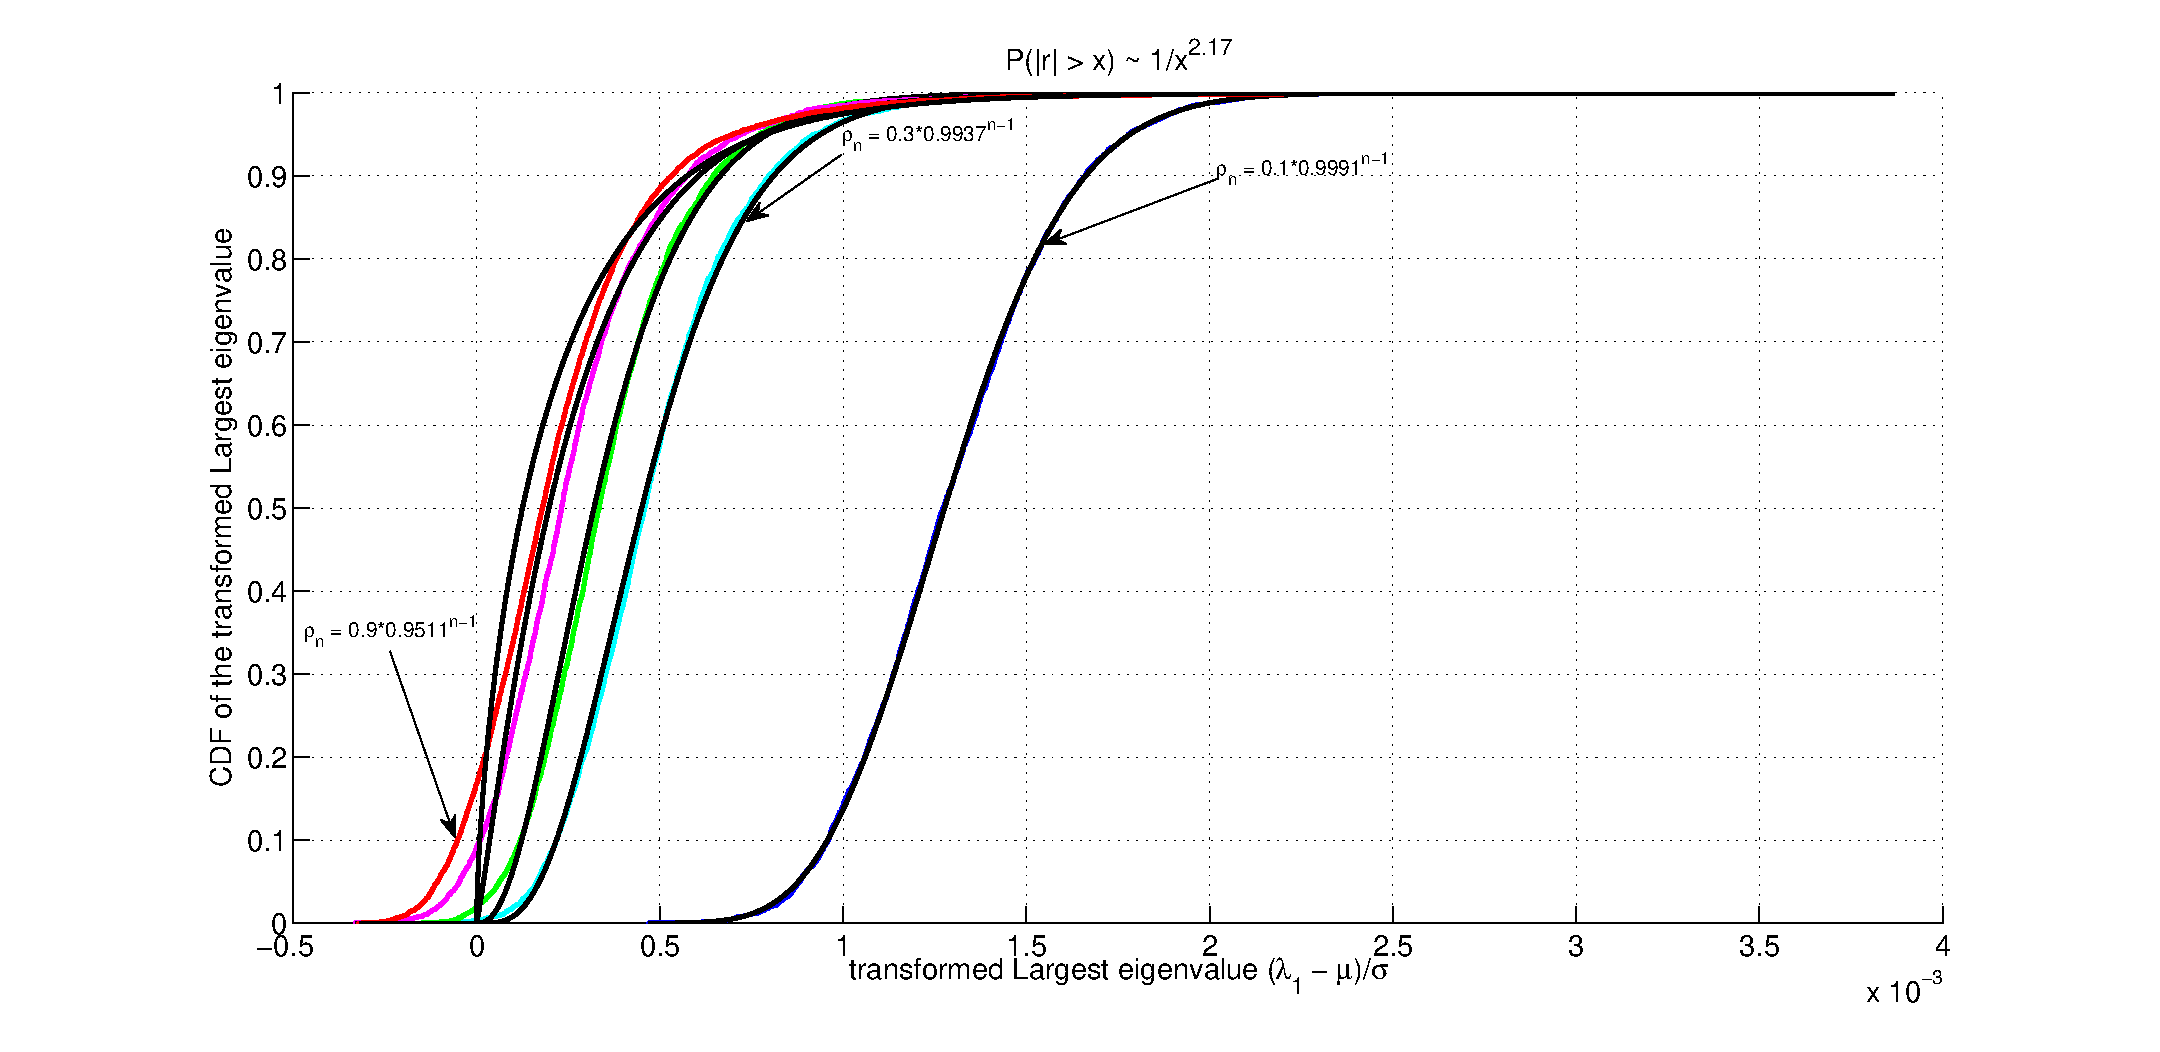
\includegraphics[scale=0.33]{../pics/maxeigen_dist_garch.eps}
    \label{fig:eig1_dist1}
  }
  \subfigure[Kolmogorov distance between the empirical cumulative
  distribution and a gamma distribution with the same mean and variance]{
    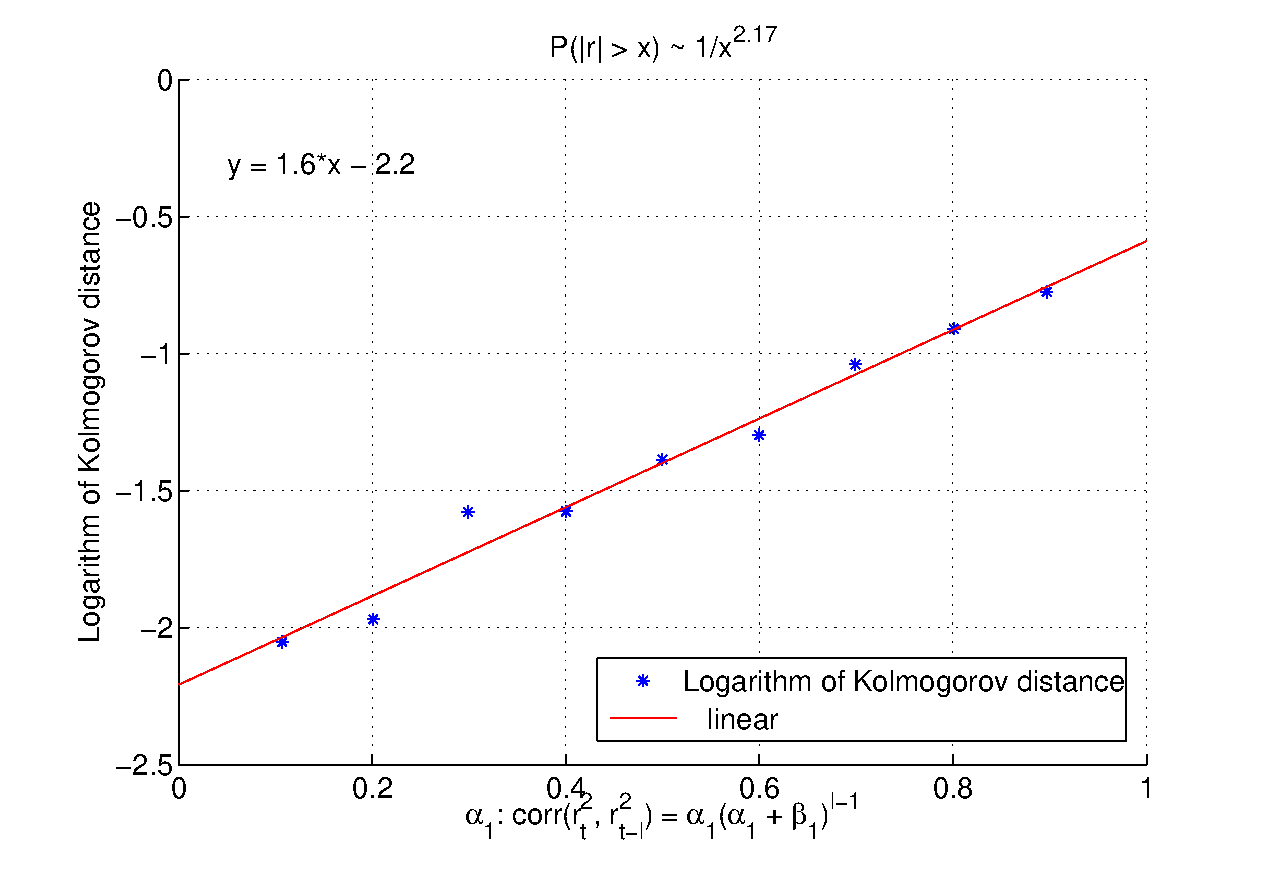
\includegraphics[scale=0.45]{../pics/maxeigen_dist_garch_ks.eps}
    \label{fig:eig1_dist2}
  }
  \caption{\small \it Distribution of the largest eigenvalue and
    comparison to a gamma distribution.}
  \label{fig:eig1_dist}
\end{figure}

Figure \ref{fig:eig1_dist3} shows the density function of the largest
eigenvalue and figure \ref{fig:eig1_dist4} shows the tail of the
complementary distribution function of the largest eigenvalue. Here by
``normalized'' we mean the following transformation:
\begin{eqnarray*}
  \lambda'_1 &=& {\lambda_1 - \E(\lambda_1) \over \text{std}(\lambda_1)}  
\end{eqnarray*}


\begin{figure}[htb!]
  \centering
  \subfigure[Probability density function of the normalized largest
  eigenvalue]{
    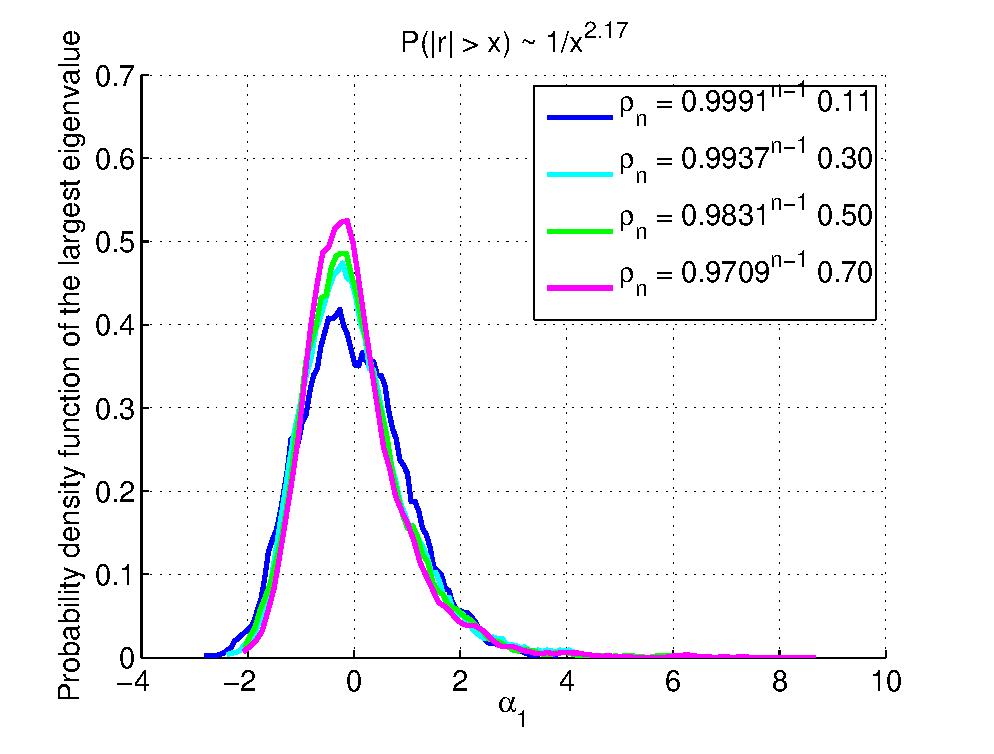
\includegraphics[scale=0.32]{../pics/maxeigen_dist_pdf.eps}
    \label{fig:eig1_dist3}
  }
  \hspace{5mm}
  \subfigure[Complementary distribution function of the
  normalized largest eigenvalue on log-log scale.]{
    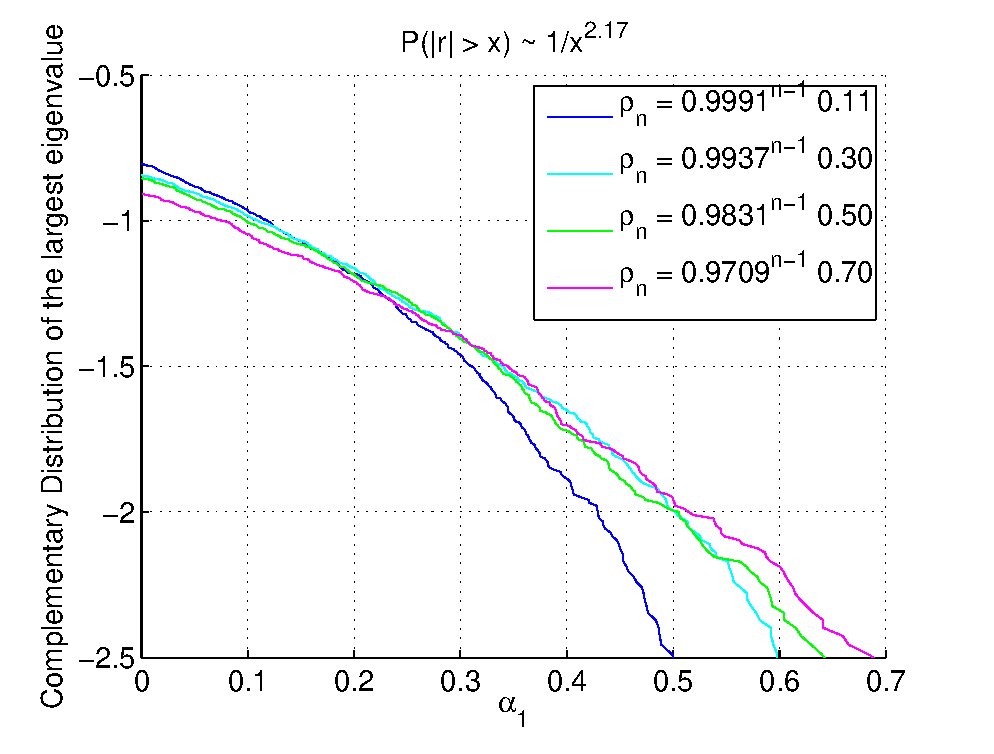
\includegraphics[scale=0.32]{../pics/maxeigen_dist_tail.eps}
    \label{fig:eig1_dist4}
  }
  \caption{\small \it Tail behavior of the largest eigenvalue.}
  \label{fig:eig1_dist_tail}
\end{figure}

\subsection{Dependence on the tail exponent}
Figure \ref{fig:eig1_dist_diff_alpha} shows how the distribution of
the largest eigenvalue depends on the tail exponent.
\begin{figure}[htb!]
  \centering
    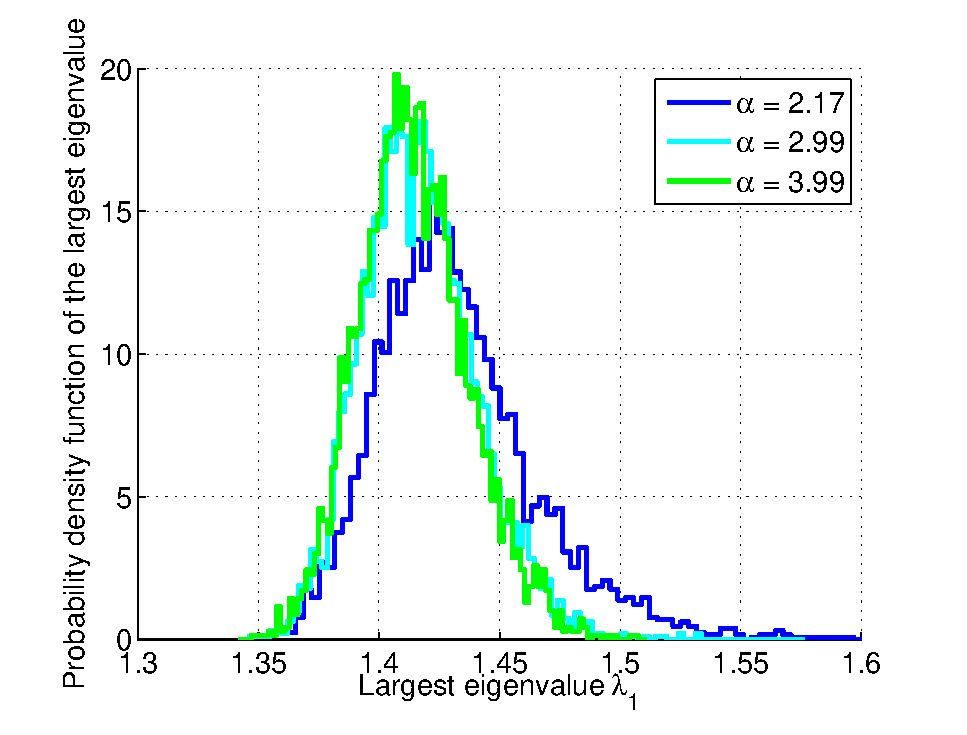
\includegraphics[scale=0.4]{../pics/eig1_dist_diff_alpha.eps}
    \caption{\small \it Dependence of the largest eigenvalue's
      probability density function on the tail exponent.}
    \label{fig:eig1_dist_diff_alpha}
\end{figure}

The mean and variance of the largest eigenvalue's distributions are
listed in table \ref{tab:eig1_dist_diff_alpha}
\begin{table}[htb!]
  \centering
  \begin{tabular}{|l|c|c|c|}
    \hline
    Tail Exponent & 2.17 & 2.99 & 3.99 \\
    \hline
    $\mean{\lambda_1}$ & 1.4306 & 1.4157 & 1.4137 \\
    \hline
    $\text{var}(\lambda_1)$ & 0.0012 & 0.0006 & 0.0005 \\
    \hline
  \end{tabular}
  \caption{mean and variance of the largest eigenvalue's distribution}
  \label{tab:eig1_dist_diff_alpha}
\end{table}


\bibliographystyle{unsrt}
\bibliography{econophysics}

\end{document}
